% 2009 年陕西卷文科第 15 题：球 O 与小圆 O1。
% 来源 PDF：普通高考/2009/2009陕西文.pdf，SHA-256 c4760285004d01aee97af7821783660b08339cca3a3fc8645052f11001ba586a。
% 原页：第 1 页（A3 三栏）第 2 栏中部，书页码 551。
% 重绘依据：球半径 2、OO1=√2，按 1 单位=1.4cm 绘制；小圆用椭圆表示，A、B 在小圆前缘。
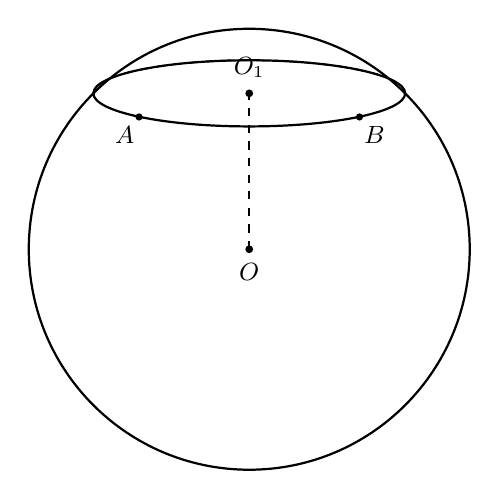
\begin{tikzpicture}[semithick, every node/.style={inner sep=1.4pt, font=\small}]
  % 球
  \draw[thick] (0,0) circle (2.8);
  % 小圆（投影为椭圆）
  \draw[thick] (0,1.98) ellipse (1.98 and 0.42);
  \draw[dashed] (1.98,1.98) arc (0:180:1.98 and 0.42);
  % 球心与小圆圆心
  \fill (0,0) circle (1.4pt);
  \fill (0,1.98) circle (1.4pt);
  \draw[dashed] (0,0) -- (0,1.98);
  % A、B
  \fill (-1.40,1.68) circle (1.3pt);
  \fill (1.40,1.68) circle (1.3pt);
  % 标注
  \node[below] at (0,-0.12) {$O$};
  \node[above] at (0,2.12) {$O_1$};
  \node[below left] at (-1.40,1.62) {$A$};
  \node[below right] at (1.40,1.62) {$B$};
\end{tikzpicture}
